\documentclass[12pt, letterpaper]{article}
\usepackage{graphicx}
\usepackage{wrapfig}
\usepackage{amsmath}
\usepackage{amssymb}
\usepackage{geometry}
\usepackage{titlesec}
\usepackage{subfiles}
\usepackage{setspace}
\usepackage{enumitem}
\usepackage[skip=0pt, indent=0pt]{parskip}
\geometry{letterpaper, portrait, margin=1in}



\begin{document}

\setlength{\parskip}{10pt}

\section*{Calculus revision 1}
Due Monday 18th August

\begin{enumerate}[itemsep=6cm]
    \item 
    \begin{enumerate}[itemsep=6cm]
        \item Find the gradient of the curve given by $y=3x^3-x^2+7$ at the point $(2, 51)$
        \item Find the x-coordinate of another point on the curve that has the same gradient as in (a).
    \end{enumerate}
    

    \item 
    Give the coordinates of the point on the curve $y=\frac{x^2}{2}+4x$ where the gradient is equal to 30.
    \pagebreak
    \item 
    Find the equation of the tangent to the curve $y=5x-2x^2$ at the point where $x=3$.
    
    \item 
    Find the equation of the tangent to the curve $y=\frac{2x^3}{3}-x^2+4x-1$ at the point $(0,-1)$

    \item 
    For what values of $x$ is the function $f(x)=4x^3+2x^2-1$ decreasing?
    \pagebreak
    \item 
    The curve $f(x)=x^3+px^2-5$ has a gradient of 20 at the point where $x=2$. Find the value of $p$.

    \item 
    A piece of cardboard is 50cm x 30cm in size. If the corners are cut out as shown below, the cardboard can be folded into an open-topped box.

    Find the maximum volume of that box.

    \begin{figure}[h]
        \centering
        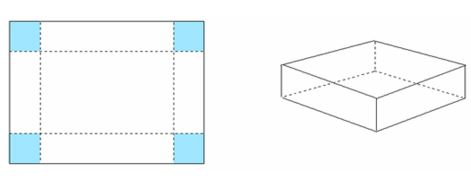
\includegraphics[width=0.5\linewidth]{images/net.png}
    \end{figure}
    Show that this is the maximum.
    \pagebreak
    \item 
    \begin{enumerate}[itemsep=6cm]
        \item 
        A car is travelling at 20 ms$^{-1}$ when the driver sees an obstruction ahead and slams on the brakes, decelerating at a rate of 2.5 ms$^{-2}$.

        How long will it take for the car to come to a complete stop? 

        \item 
        What distance will be travelled by the car before it comes to a stop?

        \item 
        If the car had less effective brakes and was only able to decelerate at 1.8 ms$^{-2}$, what is the fastest it could speed and still be able to stop in the same distance as in (b)?
    \end{enumerate}


\end{enumerate}
\end{document}
